% !TEX root = ./article.tex

\documentclass{article}

\usepackage{mystyle}
\usepackage{myvars}



%-----------------------------

\begin{document}

	\maketitle % Insert title

	\thispagestyle{fancy} % All pages have headers and footers


%-----------------------------
%	ABSTRACT
%-----------------------------

	\begin{abstract}
		\noindent [TODO ]
	\end{abstract}

%-----------------------------
%	TEXT
%-----------------------------


	\section{Introducción}
	\label{sec:introducción}

		\paragraph{}
		[TODO]

		\subsection{Perceptrón Simple}
		\label{sec:simple_perceptron}

			\paragraph{}
			[TODO ]


		\subsection{Adaline}
		\label{sec:adaline}

			\paragraph{}
			[TODO ]

	\section{Perceptrón Simple sobre conjunto de datos sencillo}
	\label{sec:e1}

		\paragraph{}
		En esta sección se describe el experimento realizado utilizando la estrategia del \emph{perceptrón simple}. El conjunto de datos utilizado se muestra en la tabla \ref{table:e1_dataset}. Este conjunto de datos posee la característica de ser linealmente separable, tal y como se verá a continuación. Está formado por \textbf{8 instancias} formadas por \textbf{2 atributos} de carácter numérico. La clase de destino también es de carácter numérico, formada por el conjunto de valores $D = \{1,-1\}$. Puesto que este conjunto está formado por dos categorías, entonces se puede utilizar un único clasificador binario (perceptrón simple en este caso) para clasificar las instancias.

		\paragraph{}
		En este caso, debido al reducido tamaño del conjunto de datos, se ha realizado un experimento basado en el error de resustitución. Por lo tanto, se ha utilizado el $100\%$ de las instancias, tando para entrenamiento como para test.

		\begin{table}[H]
			\centering
			\begin{tabu}{ | c | c | c |}
				\hline
				\multicolumn{3}{ | c | }{Simple Dataset} \\ \hline
				\bfseries $x_1$ & \bfseries $x_2$ & \bfseries $d(x)$
				\csvreader[head to column names]{../datasets/simple.csv}{
				  1=\one, 2=\two, 3=\three
				}
				{\\\hline\one&\two&\three}
				\\\hline
			\end{tabu}
			\caption{Conjunto de datos Simple}
			\label{table:e1_dataset}
		\end{table}

		\paragraph{}
		Puesto que las el conjunto de datos es linealmente separable tal y como se ha indicado anteriormente (se puede apreciar en la figura \ref{fig:e1_plot}) y la metodología experimental seguida es se apoya en el error de resustitución. La tasa de error obtenida es del $0.0\%$ tal y como se muestra en la tabla \ref{table:e1_error}.

		\begin{figure}[h]
			\begin{center}
				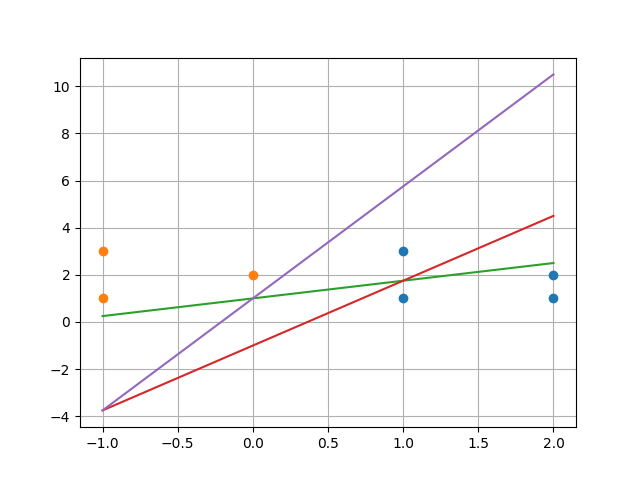
\includegraphics[width=0.75\textwidth]{simple-perceptron}
			\end{center}
			\caption{Evolución de los pesos conforme aumenta el número de iteraciones}
			\label{fig:e1_plot}
		\end{figure}

		\paragraph{}
		La figura \ref{fig:e1_plot} muestra la evolución del la recta que separa las dos clases de datos conforme aumentan las iteraciones. La línea en color \textbf{verde} se corresponde con la \textbf{iteración inicial}, la línea en color \textbf{verde} se corresponde con la \textbf{primera iteración} y, por último, la línea \textbf{púrpura} se corresponde con la \textbf{segunda iteración}. Nótese que en este punto las dos clases están separadas por dicha recta, por lo que el algoritmo ya está en codiciones de terminar.

		\begin{table}[h]
			\centering
			\small
			\begin{tabu}{ | c | c | }
				\hline
				\multicolumn{2}{ | c | }{Perceptrón Simple - Simple Dataset} \\ \hline
				Error de Resubstitucion & $0.0\%$	 \\
				\hline
			\end{tabu}
			\caption{Resultados del experimento sobre el conjunto de datos Simple}
			\label{table:e1_error}
		\end{table}

	\section{Adaline sobre Machine Dataset}
	\label{sec:e2}

		\paragraph{}
		[TODO]

		\begin{table}
			\centering
			\small
			\begin{tabu}{ | c | c | }
				\hline
				\multicolumn{2}{ | c | }{Adaline --- Machine Dataset} \\ \hline
				Error HoldOut & $71.429\%$	 \\
				\hline
			\end{tabu}
			\caption{[TODO ]}
			\label{table:e2_error}
		\end{table}

%-----------------------------
%	Bibliographic references
%-----------------------------
	\nocite{subject:taa}
  \bibliographystyle{alpha}
  \bibliography{bib/misc}

\end{document}
